% Format teze zasnovan je na paketu memoir
% http://tug.ctan.org/macros/latex/contrib/memoir/memman.pdf ili
% http://texdoc.net/texmf-dist/doc/latex/memoir/memman.pdf
% 
% Prilikom zadavanja klase memoir, navedenim opcijama se podešava 
% veličina slova (12pt) i jednostrano štampanje (oneside).
% Ove parametre možete menjati samo ako pravite nezvanične verzije
% mastera za privatnu upotrebu (na primer, u b5 varijanti ima smisla 
% smanjiti 
\documentclass[11pt,oneside]{memoir}

% Paket koji definiše sve specifičnosti mastera Matematičkog fakulteta
\usepackage{matfmaster}
\usepackage{amsmath}
\DeclareMathOperator*{\argmax}{arg\,max}
\DeclareMathOperator*{\argmin}{arg\,min}
%
% Podrazumevano pismo je ćirilica.
%   Ako koristite pdflatex, a ne xetex, sav latinički tekst na srpskom jeziku
%   treba biti okružen sa \lat{...} ili \begin{latinica}...\end{latinica}.
%
% Opicija [latinica]:
%   ako želite da pišete latiniciom, dodajte opciju "latinica" tj.
%   prethodni paket uključite pomoću: \usepackage[latinica]{matfmaster}.
%   Ako koristite pdflatex, a ne xetex, sav ćirilički tekst treba biti
%   okružen sa \cir{...} ili \begin{cirilica}...\end{cirilica}.
%
% Opcija [biblatex]:
%   ako želite da koristite reference na više jezika i umesto paketa
%   bibtex da koristite BibLaTeX/Biber, dodajte opciju "biblatex" tj.
%   prethodni paket uključite pomoću: \usepackage[biblatex]{matfmaster}
%
% Opcija [b5paper]:
%   ako želite da napravite verziju teze u manjem (b5) formatu, navedite
%   opciju "b5paper", tj. prethodni paket uključite pomoću: 
%   \usepackage[b5paper]{matfmaster}. Tada ima smisla razmisliti o promeni
%   veličine slova (izmenom opcije 12pt na 11pt u \documentclass{memoir}).
%
% Naravno, opcije je moguće kombinovati.
% Npr. \usepackage[b5paper,biblatex]{matfmaster}

% Pomoćni paket koji generiše nasumičan tekst u kojem se javljaju sva slova
% azbuke (nema potrebe koristiti ovo u pravim disertacijama)
\usepackage{pangrami}

% Paket koji obezbeđuje ispravni prikaz ćiriličkih italik slova kada
% se koristi pdflatex. Zakomentarisati ako na sistemu koji koristite ovaj
% paket nije dostupan ili ako ne radi ispravno.
\usepackage{cmsrb}

% Ostali paketi koji se koriste u dokumentu
\usepackage{listings} % listing programskog koda
\usepackage{hyperref}

% Ime kandidata na srpskom jeziku (u odabranom pismu)
\autor{Момир Аџемовић}
% Naslov teze na srpskom jeziku (u odabranom pismu)
\naslov{Предикциjа траjекториjа више обjеката на сцени}
% Godina u kojoj je teza predana komisiji
\godina{2022}
% Ime i afilijacija mentora (u odabranom pismu)
\mentor{др Младен Николић, ванредни професор\\ Универзитет у Београду, Математички факултет}
% Ime i afilijacija prvog člana komisije (u odabranom pismu)
\komisijaA{др Јована Ковачевић, доцент\\ Универзитет у Београду, Математички факултет}
% Ime i afilijacija drugog člana komisije (u odabranom pismu)
\komisijaB{др Александар Картељ, доцент\\ Универзитет у Београду, Математички факултет}
% Ime i afilijacija trećeg člana komisije (opciono)
% \komisijaC{}
% Ime i afilijacija četvrtog člana komisije (opciono)
% \komisijaD{}
% Datum odbrane (obrisati ili iskomentarisati narednu liniju ako datum odbrane nije poznat)
\datumodbrane{15. септембар 2022.}

% Apstrakt na srpskom jeziku (u odabranom pismu)
\apstr{%
У изради...
}

% Ključne reči na srpskom jeziku (u odabranom pismu)
\kljucnereci{машинско учење, аутономна вожња, растеризација, графовске неуронске мреже}

\begin{document}
% ==============================================================================
% Uvodni deo teze
\frontmatter
% ==============================================================================
% Naslovna strana
\naslovna
% Strana sa podacima o mentoru i članovima komisije
\komisija
% Strana sa posvetom (u odabranom pismu)
\posveta{посвета... у изради...}
% Strana sa podacima o disertaciji na srpskom jeziku
\apstrakt
% Sadržaj teze
\tableofcontents*

% ==============================================================================
% Glavni deo teze
\mainmatter
% ==============================================================================

% ------------------------------------------------------------------------------
\chapter{Увод}
% ------------------------------------------------------------------------------

TODO: ...

\section{Поставка проблема}

Предвиђање трајекторија или предвиђање кретања једног агента на сцени са више покретних објеката (суседи аналогни агенту) се формално
дефинише као предикција скупа вредности $\{(x^{t}_a, y^{t}_a)\ |\ t \in [0, T]\}$, где је $T$ дужина трајекторије агента која се предвиђа, 
под претпоставком да су дате следеће информације:
\begin{itemize}
  \item Историја тог агента $А_{h} = \{(x^{t}_a, y^{t}_a)\ |\ t \in [-H, -1]\}$, где је $H$ дужина историје трајекторије;
  \item Историја осталих покретних агената $\{T^{n}_{raj}\ |\ n \in N\}$, где је $T^{n}_{raj}$ истог облика као и $A_{h}$, а $N$ је скуп
        свих суседа;
  \item Окружење агента $E$ - варира у односу на скуп података.
\end{itemize}

\section{Опис података}

Мапа са високим нивоом детаља (\textit{eng. HD map}) је мапа путева са прецизношћу до пар центиметара и високим нивоом
познавања окружења: позиције пешачких прелаза, позиције семафора, полигони путева, смерови улица итд... Битно је нагласити
да су \textit{HD} мапе супериорне у односу на \textit{GPS} у смислу прецизности и разноврсности информација. Саме \textit{GPS}
мапе нису довољно прецизне да може да их користи систем за аутономну вожњу уместо људи који су значајно робуснији на грешке
\textit{GPS}-a (што може да буде и до неколико метара). Аналогија HD мапа са човеком и вожња добро познатим путем и вожња 
непознатим путем први пут у животу. Вожња добро познатим путем одговара знању које се добија из HD мапа. 


Овај тип података даје јако велику количину информација које се могу процесирати у целокупном систему аутономне вожње. Два главна проблема
и изазова овог типа података је њихово прикупљање (LiDAR системи су скупи) и одржавање, и обрада овако неструктуираних података. Алтернатива
је коришћење камера и модела дубоког учења за прикупљање података о окружењу у реалном времену (Теслин присуп - ТОДО: Додати референцу), које
делимично може да замени HD мапе. 

\chapter{Преглед претходних приступа}
\label{chp:razrada}
% ------------------------------------------------------------------------------

TODO: Средити одређене делове да текст буде јаснији...

Техника за предикцију трајекторија више објеката које издвајају посебан објекат као агент, могу да се групишу грубо у четири групе. Постоје
и општије технике које не разликују конкретно агента од осталих објеката у процесу предвиђања.

\section{Опште технике које не издвајају одређени објекат као агента}

Неке од првих метода за предикцију трајекторија, јесу рекурентне неуронске мреже 
(\textit{eng. RNN - Recurrent neural network}) и конволутивне мреже за једну димензију (\textit{CNN - Convolutional Neural Network}). 
Често је коришћена \textit{LSTM} архитектура рекурентних неуронских мрежа погодна за коридање динамике објеката. 
Како трајекторија једног објекта зависи од трајекторија осталих објеката,
неопходно је да се користи некакав механизам пажње којим се добија веза између различитих објеката на сцени. \cite{argoverse} \cite{social_lstm} 
Мана овог скупа модела је што модели нису погодни за потпуно разумевање веза између различитих елемената сцена (објекти, возне линије, саобраћајни знакови, ...).

Уместо учења модела који дају предикције трајекторија које се у просеку најбоље у тим случајевима, 
алтернатива су скуп архитектура заснованих на (условљеним) генеративним моделима који
омогућавају генерисање произвољог броја трајекторија, као узорковање из условљене расподеле (расподела је условљена историјом трајекторије, као и
окружењем у којем се тај објекат налази). Пример је \textit{Social GAN} \cite{social_gan} архитектура која узима у обзир претходне наведене услове и генерише ,,социјално прихватљиве`` трајекторије
пешака. Један од главним мотива ових мрежа је одговор на проблем мултимодалности расподела трајекторија. 
У случају возила са агентом, генеративни модели захтевају током процеса предикције напредније алгоритме узорковања ради оптимизације покривености
трајекторијама\footnote{Покривеност се односи на метрике које узимају у обзир више од једне трајекторије, па је битно и да те
саме трајекторије буду разноврсне}.

\section{Технике засноване на растеризацији}

Растеризација подразумева трансформацију \textit{HD} мапа у формат слике. Слике приказују сцене из птичје перспективе (\textit{eng. BEV - Bird's-eye-view}).
Предност овог формата је могућност примене више слојева конволутивних неуронских мрежа за извлачење 
контекста тих мапа. Овакве компоненте архитектуре се углавном називају енкодери. Конволутивне мреже нису ограничене да раде са RGB 
и сличним форматима слика тј. сваком пикселу може да се додели низ својстава. Нека од очигледнијих својстава су: да ли агент заузима тај пиксел, 
да ли сусед (неагент) заузима тај пиксел,
да ли пиксел припада улици, ... Излаз CNN енкодера се углавном накнадно комбинује са осталим компонентама за генерисање резултата. 

Излази модела такође могу да се представљају као слике тј. топлотне мапе \textit{(eng. Heat Map)}, где се сваком пикселу додељује вероватноћа
да се агент (или посматрани објекат) налази на тој локацији. Топлотне мапе се добијају декодерима који комплементирају енкодер компоненте.
То значи да није неопходно да се експлицитно постави ограничење на одређени број излазних трајекторија модела. Проблем
код више излазних трајекторија модела је то што може да изазове колапс моде (eng. \textit{mode collapse}). Број трајекторија се овде не 
дефинише експлицитно и може да варира од једне сцене до друге. Наравно, не узимају се сви пиксели као кандидати, већ се примењује неки
алгоритам узорковања. \cite{home} \cite{centernet}

Архитектура \textit{HOME} \cite{home} користи овај принцим за паралелно кодирање растеризоване сцене и трајекторија oбјеката. Резултати
компоненти се спајају и прослеђују као улаз у декодер за генерисање топлотне мапе. Узорковањем тачака из топлотних мапа се добија скуп кандидата тачака.
Главна претпоставка архитектура заснованих на топлотним мапама је: Ако знамо циљну тачку и историју трајекторије објекта, онда можемо
једноставно да одредимо трајекторију до те циљне тачке. За одређивање ових трајекторија могу да се користе једноставнији модели неуронских мрежа.

Могуће је растеризовати потпуно податке тј. растеризовати и трајекторије као низ слика. Свака слика садржи скуп тачака које представљају
локације објеката. Архитектура \textit{CASPNet} \cite{caspnet} примењује CNN енкодер на свако стање и користи ConvLSTM \cite{convlstm} за разумевање
темпоралних веза. На овај начин се извлаче својства динамичког дела сцена. На сличан начин је могуће и извући својства и за 
статички део (возне линије, возни површине, ...) користећи класичне конволутивне мреже. Комбинацијом ових података се генеришу
трајекторије које су исто у растеризованом облику.

\section{Технике засноване на графовским репрезентацијама}

Мапе имају комплексну топологију. Технике засноване на растеризацији користе конволуцију која тешко 
извлачи потпуно семантику тих мапа. Алтернатива је моделовање мапа графовским структурама. 
Технике засноване на графовском репрезентацијом као улаз добијају стање мапе кодиране као граф и примењују моделе графовских неуронских мрежа. 
Две архитектуре које представљају основе за већину архитектура ове групе су \textit{LaneGCN} \cite{lanegcn} и \textit{VectorNet} \cite{vectornet}.

Мапа може да се моделује као скуп повезаних сложених линија (\textit{end. polylines}), где сваком објекту одговара једна усмерена сложена линија. 
\textit{VectorNet} је хијерархијска графовска неуронска мрежа која као улаз добија мапу која је моделована као скуп 
сложених линија, а као резултат даје скуп предикција трајекторија. Идеја је да се прво извуку својста из сложених 
линија појединачних објеката, а онда то пронађу одговарајуће везе између између објеката међусобно и између објеката и возних линија. \cite{vectornet} 

Архитектура \textit{LaneGCN} нуди варијанту конволутивних графовских мрежа (\textit{GCN - Graph Convolution Network}) 
која је специјализована за графове возних линија које имају различите типове веза. Користе се различите матрице
повезаности за суседе, претходнике, следбенике (леви и десни). За сваку матрицу повезаности може да се примени класичан GCN, а
комбиновањем тих елемената је добија један LaneGCN слој. \cite{lanegcn} 

\section{Хибридне технике}

Хибридне технике користе комбинацију структура графова и BEV слика. \textit{GOHOME} Модификована верзија \textit{HOME} која уместо
CNN енкодера и растеризованих слика мапа, користи \textit{LaneGCN} архитектуру за енкодер. Заправо ансамбл ова два модела (\textit{HOME, GOOME})
даје најбоље резултате по \textit{MR} метрици\footnote{Објашњење за ову метрике се налази у секцији за евалуацију}.

\section{Технике засноване на облацима тачака}

Последња група нешто одступа од осталих али и даље даје добре резултате. Подаци се посматрају као облаци тачака (\textit{eng. point cloud}) 
и примењују се технике намењене за такву структуру података. Основна
архитектура је \textit{TPCN} \cite{tpcn} која је заснована на \textit{PointNet} \cite{pointnet}, а већина осталих техника су ,,изведене``.

% ------------------------------------------------------------------------------
\chapter{Припрема података}

Основни скуп података за тренирање и тестирање техника предикције трајекторија је \textit{Argoverse Motion Forecasting} скуп података
који се састоји од 324 хиљаде детаљних мапа саобраћаја (\textit{eng. ,,HD maps``}) које садрже геометријске и семантичке податке сцена. Постоје две \textit{HD} сцене
за градове Питсбург и у Мајами. Коришћењем аутономних возила су генерисани сценарији који представљају неколико узастопних слика сцена (у табеларном формату)
на деловима мапа. Сви детаљи о овом скупу података се могу пронаћи на адреси 
\href{https://www.argoverse.org/index.html}{\color{blue}{www.argoverse.org}} \cite{argoverse}. \\


\noindent Kључне информације које се издвајају из сваког сценарију су:
\begin{itemize}
  \item Мапа сценарија (Питсбург или Мајами);
  \item Трајекторије агената;
  \item Трајекторије осталих објеката на сцени;
  \item Возне (централне) линије.
\end{itemize}

\section{Претпроцесирање података}

\noindent Подаци сваког сценарија се векторизују и чувају у полу-структуираном формату. 
За парсирање и обраду улазних података се користи \textit{argoverse API} интерфејс.


Трајекторија агента\footnote{Низ $(x, y)$ тачака, где је приближна временска разлика између две тачке око 0.1 секунде} 
се дели на два дела: историја (својства) и реализација (будуће вредности). Реализација се састоји од $N_r$ 
опажања $x$ и $y$ релативних координата\footnote{Све координате се нормализују тако да су релативне у односу на последње опажање у трајекторији историје агента} 
тј. облик реализације је $(N_r, 2)$. 
Историја се аналогно формира да садржи историју $N_h$ опажања $x$ i $y$ релативних координата. Овај део трајекторије иде непосредно
пре реализације. Посматрамо следеће случајеве:
\begin{itemize}
  \item Постоји више од $N_h + N_r$ опажања: Одбацује се реп трајекторије (првих неколико вредности хронолошки гледано);
  \item Постоји мање од $N_{hmin} + N_r$ опажања: Сценарио се одбацује (сматра се да је невалидан);
  \item Постоји између $N_{hmin} + N_r$ и $N_h + N_r$ опажања: реп трајекторије се допуњава до димензије $N_h + N_r$ 
  посматрано као да објекат мирује у тим тренуцима.
\end{itemize}
Коначно, облик историје је $(N_h, 3)$, где трећа вредност означава да ли је опажање право ($1$) или допуњено ($0$).

Трајекторије суседних објеката се деле на два дела аналогно трајекторији агента. Неопходно је да се синхронизују трајекторије 
суседних објеката по временским ознакама (eng. \textit{timestamp}) са трајекторијом агента, јер не постоји у сваком тренутку исти
број објеката на сцени. Након синхронизације се трајекторије деле на историју и реализацију и проверава се да ли дужине тих
делова задовољавају критеријуме:
\begin{itemize}
  \item Уколико је дужина трајекторије историје краћа од $N_{homin}$, онда се објекат одбацује;
  \item Уколико је дужина трајекторије реализације краћа од $N_{romin}$, онда се објекат одбацује.
\end{itemize}
Као додатна провера, за сваки сусед се провера растојање од агента. Уколико је сусед превише далеко, онда се се он одбацује.
Критеријум за одбацивање суседа узима у обзир брзину агента (по $x$ и $y$ оси одвоједно) и растојање њихових последњих опажања
у трајекторији историје. Уколико неки од следећих услова није
испуњен, сусед се игнорише у сценарију: $\frac{O_n^x}{A_s^x} \leq T_{steps}$, $\frac{O_n^y}{A_s^y} \leq T_{steps}$,
где је $O_n^x$ ($O_n^y$) нормализована $x$ ($y$) координата суседа, $А_s^x$ ($А_s^y$) је наивно 
апроксимирана\footnote{Брзина се апроксимира као просек промена координата у трајекторији историје} брзина агента
по $x$ ($y$) оси и $T_{steps}$ је параметар толеранције.
Трајекторије се секу или допуњавају до фиксног облика. Векторизован облик: $(N_n, N_h, 3)$ и $(N_n, N_r, 3)$, где је $N_n$ број
судедних објеката. 

На основу локације агента се издвајају сегменти централних линија (возне путање) које нису даље од агента за више од $D_{lsinit}$. Уколико нема
пронађених сегмената централних линија, онда се вредност за $D_{lsinit}$ множи $K_{ls}$\footnote{$D_{lsinit}$ и $K_{ls}$ су фиксне вредности
у \textit{argoverse} интерфејсу} 
пута до највише $D_{lsmax}$ (ако и даље нема сегмената, 
онда се сценарио одбацује). За сваки сегмент се чува низ од 10 $(x, y)$ координата приширених са метаподацима:
\begin{itemize} 
  \item \textit{is\_intersection} - да ли се сегмент сече са неким сегментом,
  \item \textit{turn\_right} - да ли је у питању скретање у десно, 
  \item \textit{turn\_left} - да ли је у питању скретање у лево, 
  \item \textit{turn\_none} - да ли нема стретања, 
  \item \textit{is\_traffic\_control} - да ли постоји контрола саобраћаја. 
\end{itemize}
Коначан облик је $(N_{ls}, 10, 7)$. 

Скуп кандидата централних сегмената линија за предикције трајекторија: Постоји коначан број централних сегмената линија по којој
објекат може да се креће у скоријој будућности, због чега је корисно да се као улаз у модел користе централне линије као кандидати. 
Основа алгоритма за проналазак ових кандидата се налази у \textit{argoverse} интерфејсу \cite{argoverse}. Кандидати се проналазе
коришћењем трајекторије историје агента. Коначан векторизован облик је: $(N_c, N_r, 3)$, где је $N_c$ број пронађених кандидата,
$N_r$ дужина трајекторије реализације. Пошто се централне линије допуњавају по потреби до димензије $N_r$, користи се трећа координата
за маску. Погледати табелу \ref{dp-params-table} за преглед свих параметара процеса.

\begin{table}
  \begin{tabular}{c|c}
    Ознака параметра & Објашњење \\
    \hline
    $N_r$ & Дужина трајекторије реализације (део који се предвиђа) \\
    $N_h$ & Дужина трајекторија историје \\
    $N_{hmin}$ & Минимална дужина трајекторије историје пре допуњавања \\
    $N_{hоmin}$ & Минимална дужина трајекторије историје суседа пре допуњавања \\
    $N_{rоmin}$ & Минимална дужина трајекторије реализације суседа пре допуњавања \\
    $T_{steps}$ & Умножак максималног растојања до сегмента централне линије \\
    $D_{lsmax}$ & Максимално растојање до централне линије
  \end{tabular}
  \caption{Преглед параметара припреме података}
  \label{dp-params-table}
\end{table}

На сликама \ref{scenario-example-3700} и \ref{scenario-example-4791} се налазе примери два визуализована сценарија
након претходне припреме. У овом формату нису прикази делови сцене на којој је могућа вожња, али 
постоје (централне линије) тј. путање по којима се возила најчњшће крећу. Изузеци су у случају неких скретања,
промени линија, ...

\begin{figure}[h!]
  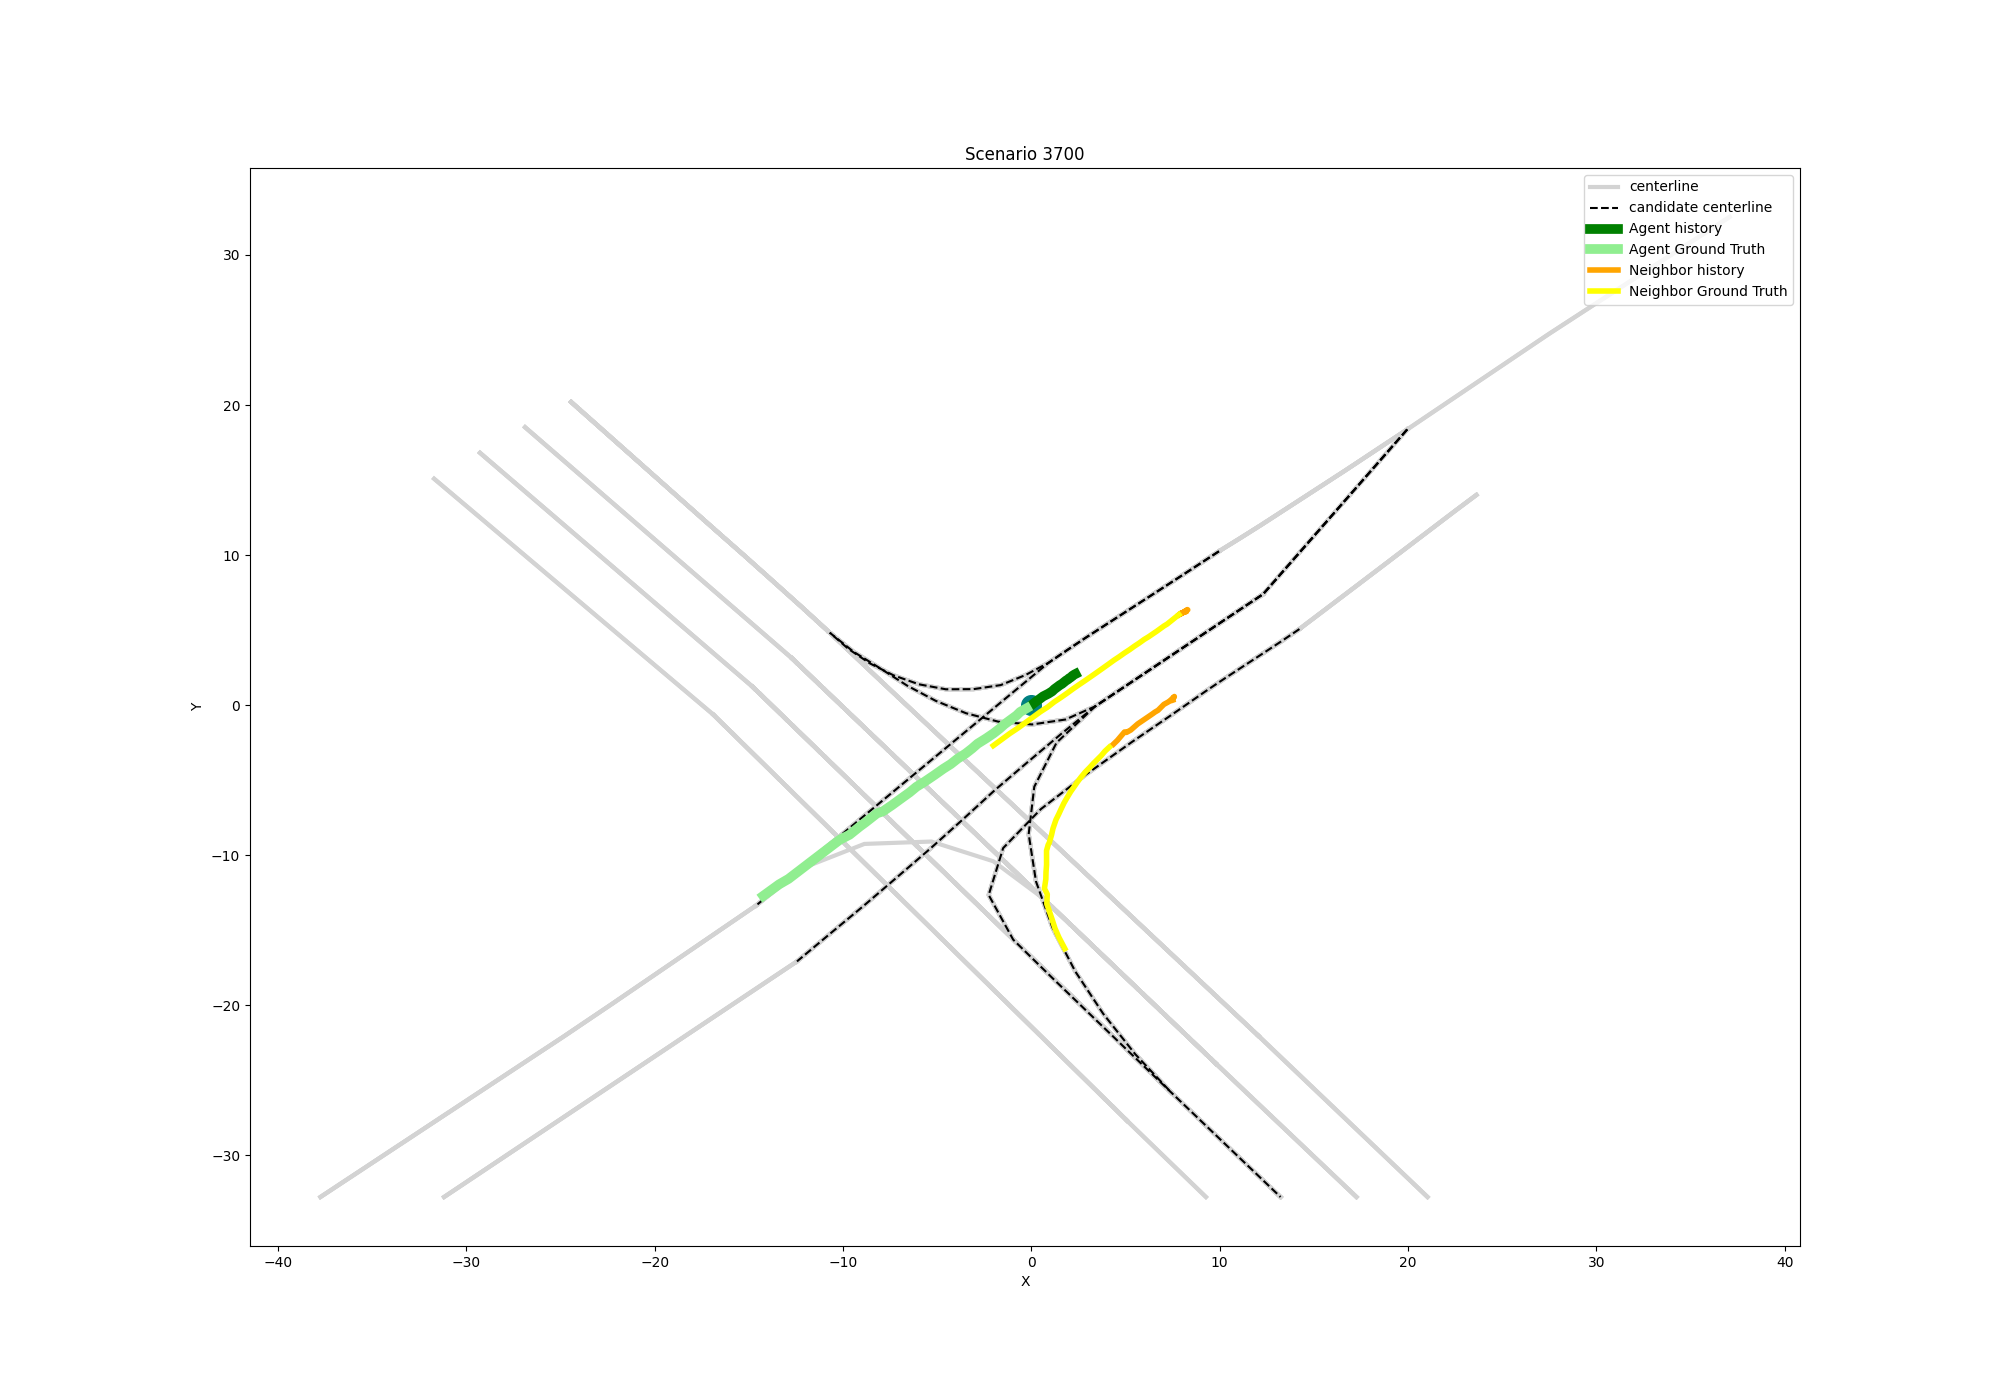
\includegraphics[width=0.9\textwidth]{images/scenario3700.png}
  \caption{Визуализација припремљених података - Пример 1}
  \label{scenario-example-3700}
\end{figure}

\begin{figure}[h!]
  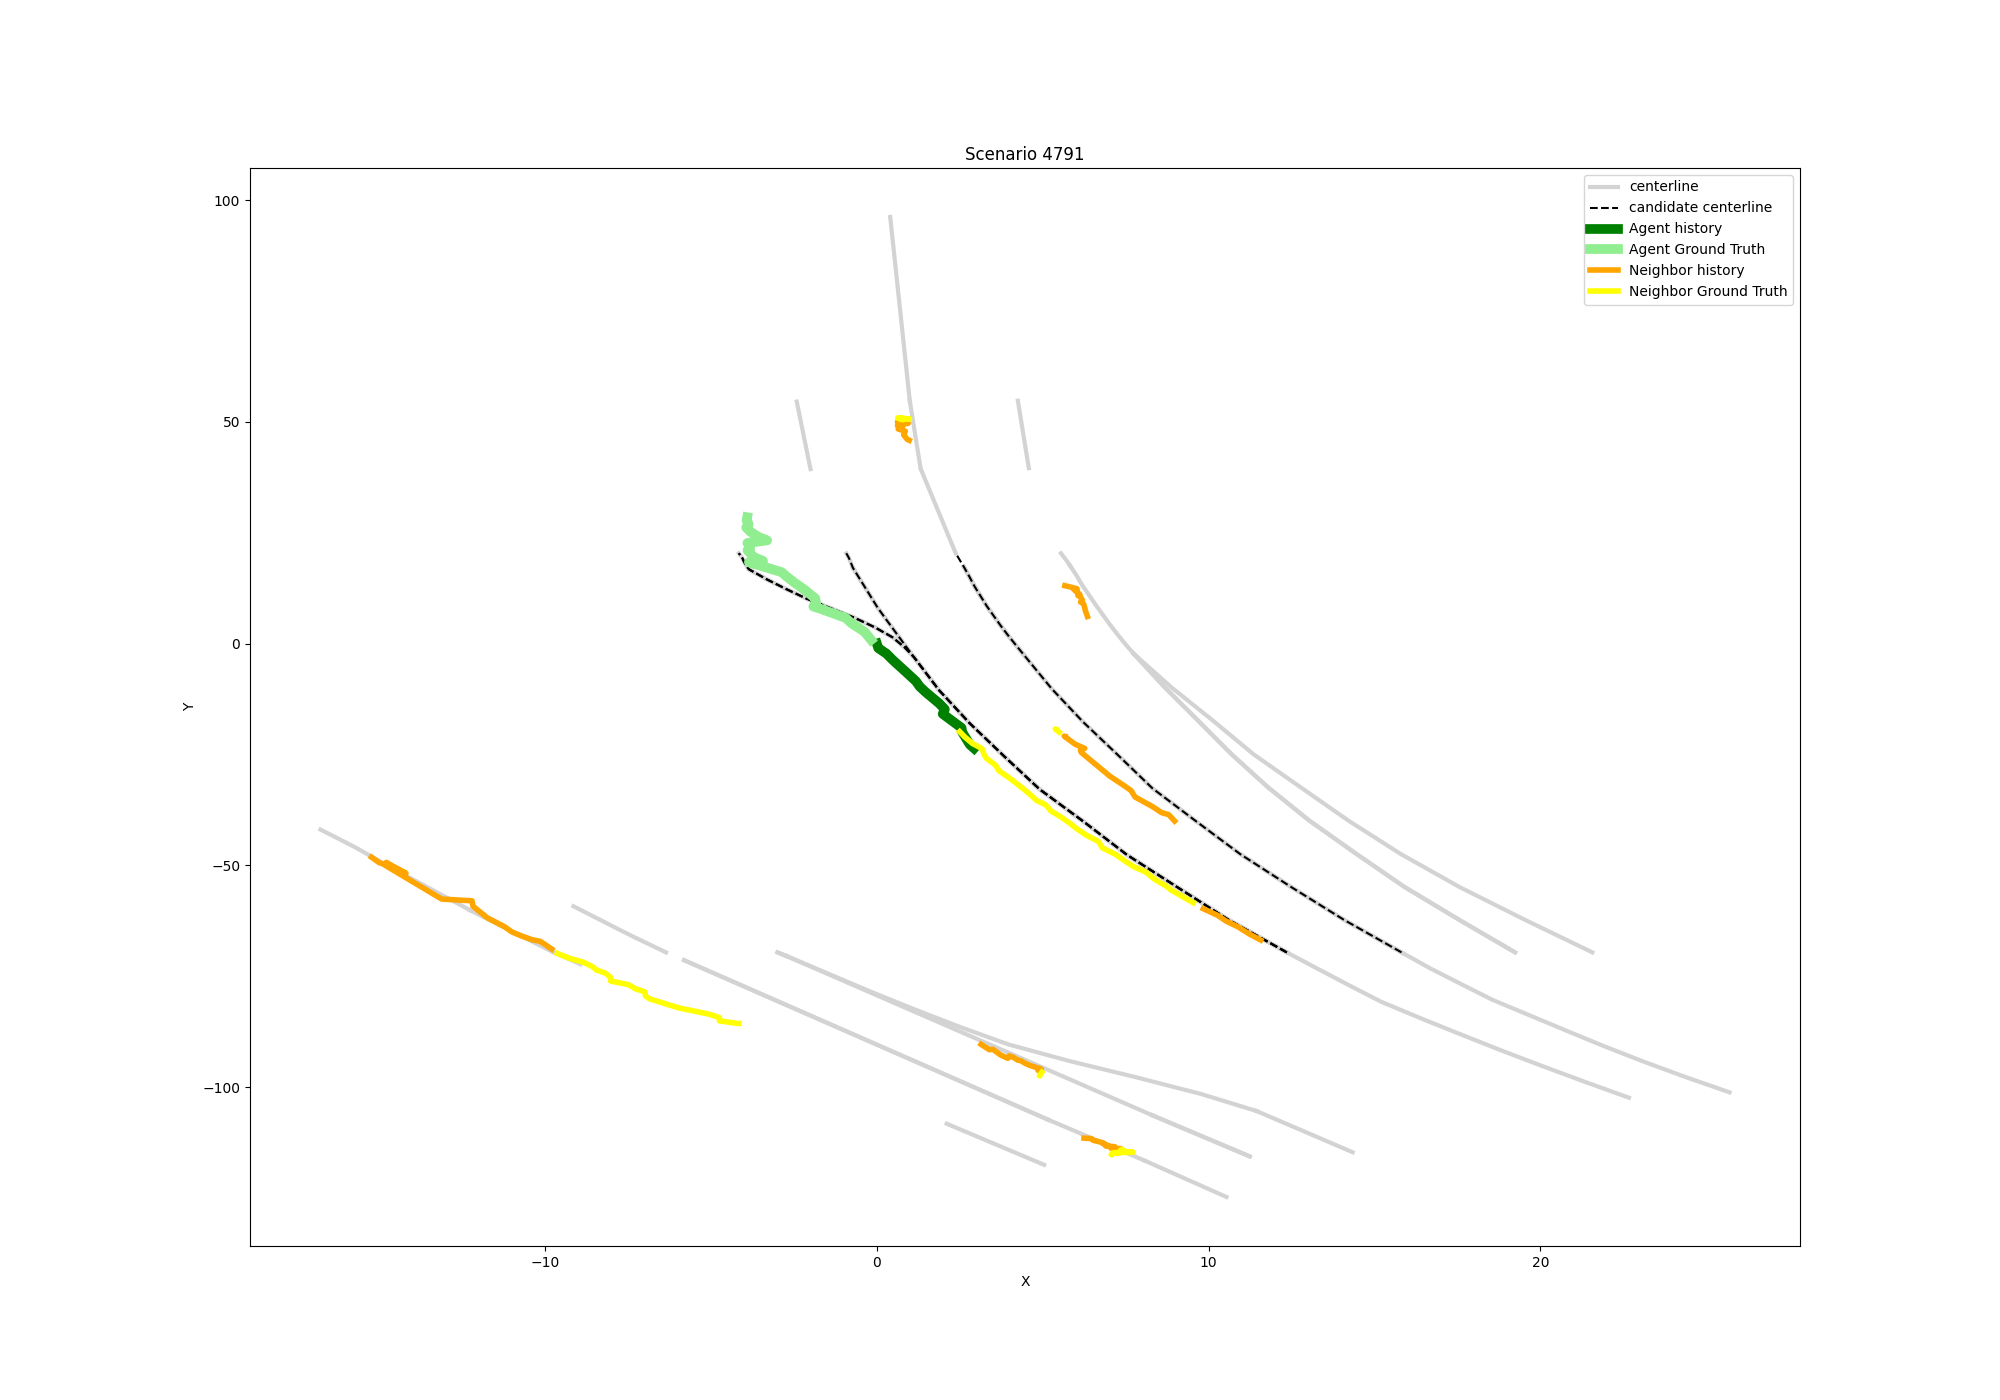
\includegraphics[width=0.9\textwidth]{images/scenario4791.png}
  \caption{Визуализација припремљених података - Пример 2}
  \label{scenario-example-4791}
\end{figure}


% ------------------------------------------------------------------------------
\chapter{Преглед метода за евалуацију модела}
\label{chp:razrada}
% ------------------------------------------------------------------------------

Неке од стандардних метрика за евалуацију квалитета предикције трајекторија су ,,просечнa грешка одступања`` (\textit{eng. ADE - Average Displacement Error})
и ,,последња грешка одступања`` (\textit{eng. FDE - Final Displacement Error}). У наставку се користе енглеске скраћенице \textit{ADE} и
\textit{FDE}. Метрика \textit{ADE} се добија
упросечавањем еуклидског растојања између временски синхронизованих тачака трајекторија предикције и реализације. 
Метрика \textit{FDE} узима у обзир само последњу тачку. \cite{social_gan} \cite{argoverse} 
У наставку се налазе формуле у случају да се посматра тачно један објекат (нпр. само агент):

\begin{figure}[h!]
  \centering
  $ADE = \frac{1}{T}\sum_{k=1}^{T}\sqrt{(x_k - \hat{x}_k)^2 + (y_k - \hat{y}_k)^2}$
\end{figure}

\begin{figure}[h!]
  \centering
  $FDE = \sqrt{(x_{last} - \hat{x}_{last})^2 + (y_{last} - \hat{y}_{last})^2}$
\end{figure}

Метрике се једноставно уопштавају у случајевима где постоји више објеката на сцени:

\begin{figure}[h!]
  \centering
  $ADE = \frac{1}{T\times N}\sum_{n=1}^{N}\sum_{k=1}^{T}\sqrt{(x^n_k - \hat{x}^n_k)^2 + (y^n_k - \hat{y}^n_k)^2}$
\end{figure}

\begin{figure}[h!]
  \centering
  $FDE = \frac{1}{N}\sum_{n=1}^{N}\sqrt{(x^n_{last} - \hat{x}^n_{last})^2 + (y^n_{last} - \hat{y}^n_{last})^2}$
\end{figure}

Ове једноставне метрике су погодне када претпостављамо да је расподела трајекторија унимодална тј. природа трајекторија је претежно детерминистичке. 
Неки скуповима података трајекторија имају јачу стохастичку природу због стохастичке природе самих објеката (трајекторија) или непотпуних опажања окружења. 
Пример таквог скупа података је скуп трајекторија пешака. Пешак који је прешао пешачки прелаз, може у том тренутку да скрене лево или десно.
У том случају имају два вероватна сценарија за исту историју трајекторије (углавном немамо информације о циљевима самог пешака). \cite{social_gan} \cite{best_of_many_cvae}

Скуп ,,најбољи из групе`` (\textit{eng. ,,Best of Many``}) техника узимају у обзир мултимодалну природу расподела трајекторија. Модел може
да генерише неколико различитих предикција трајекторија и за сваку трајекторију одговарајућу вероватноћу (поузданост). Као грешка се узима предикција
која је најбоља по дефинисаном критеријуму (критеријум не мора да се поклапа са самом мером која се користи). \cite{best_of_many_cvae} \cite{argoverse}
Претходно наведене технике \textit{ADE} и \textit{FDE} се уопштавају у \textit{minADE} и \textit{minFDE}. Због једноставности узимају се у обзир облици
са једним објектом: \cite{Disdis} \cite{best_of_many_cvae}

\begin{figure}[h!]
  \centering
  $minADE = ADE(\displaystyle\argmin_{\hat{T}^k_{raj}} FDE(\hat{T}^k_{raj}, T_{raj}), T_{raj}), k \in \{1, ..., K\}$ 
\end{figure}

\begin{figure}[h!]
  \centering
  $minFDE = \displaystyle\min FDE(\hat{T}^k_{raj}, T_{raj}), k \in \{1, ..., K\}$
\end{figure}

Уколико модел генерише више од \textit{K} трајекторија, узима се и обзир првих \textit{K} по поузданости. У специјалном случају када је $K = 1$, онда 
\textit{minFDE} постаје \textit{FDE}, а \textit{minADE} се и даље разликује по избору ,,главне`` трајекторије. 
Проблем са \textit{minADE} i \textit{minFDE} је у томе што не узимају у обзир остале трајекторије поред најбоље и самим тим се не прави разлика
између предикције са свим добрим трајекторијама и предикције са једном добром трајекторијом. \cite{Disdis} 
Друга замерка овим метрикама је што не узимају у обзир поузданост предикција након филтрирања \textit{K} трајекторија. Уколико је најбоља трајекторија
прецизна, желимо и даље да знамо да ли је модел сигуран или је добар резултат последица ,,среће``. Модификоване метрике: \cite{home}

\begin{figure}[h!]
  \centering
  $p\mbox{--}minADE = ADE(\hat{T}^{min}_{traj}, T_{raj}) - \ln{P(\hat{T}^{min}_{traj}|E_{nv})}$
\end{figure}

\begin{figure}[h!]
  \centering
  $p\mbox{--}minFDE_{prob} = FDE(\hat{T}^{min}_{traj}, T_{raj}) - \ln{P(\hat{T}^{min}_{traj}|E_{nv})}$
\end{figure}

Овде је $\hat{T}^{min}_{traj}$ трајекторија која има најбољу $FDE$ оцену, а $p(\hat{T}^{min}_{traj}|E_{nv})$ је условљена вероватноћа те 
трајекторије у односу на стање окружења. Уколико метрика \textit{ADE} (\textit{FDE}) има малу вредност за одговарајућу трајекторију, али њена одговарајућа вероватноћа има малу вредност, 
онда негативан логаритам те вероватноће има велику вредност. \cite{argoverse} У импементацији се ова вероватноћа ограничава са доње стране, како не
би дошло до прекорачења због велике апсолутне вредности након примене логаритма на веома мале вредности.

Уместо упросечавања \textit{L2} растојања у сваком кораку, могу да се броје кораци у којима трајекторије одступају за више од $MR_{thresh}$. 
Мотивација за ову метрику је чињеница да одступање које је 1 или 2 метра од реализације није толико релевантно у односу на 
велику разлику одступања. \cite{home} Такође постоји верзија метрике која узима у обзир вероватноћу и кажњава предикцију 
модела ако је добра, а модел је ипак несигуран.

\begin{figure}[h!]
  \centering
  $MR = \sum^T_{k=1} I(||\hat{T}^{k}_{traj} - T_{raj}||_{2} \geq MR_{thresh})$
\end{figure}

\begin{figure}[h!]
  \centering
  $MR_{prob} = \sum^T_{k=1} I(||\hat{T}^{k}_{traj} - T_{raj}||_{2} \geq MR_{thresh}) $
  $+ I(||\hat{T}^{k}_{traj} - T_{raj}||_{2} < MR_{thresh}) \cdot (1.0 - P(\hat{T}^{k}_{traj}|E_{nv}))$
\end{figure}

\noindent У случају \textit{Argoverse} скупа података, за параметар $MR_{thresh}$ се узима 4 пиксела тј. 2 метра у реалном свету. 

Све до сада наведене метрике су опште примене на било које објекте за које се предвиђају трајекторије. Пошто је агент увек возило, може да
се анализира да ли предикцијa трајекторија скреће са пута. Због тога се уводи метрика ,,сагланост са продучјем вожње`` 
(\textit{eng. DAC - Drivable Area Compilance}), која одређује учесталост трајекторија које нису скренуле са пута од изабраних 
\textit{K} трајекторија: \cite{argoverse}

\begin{figure}[h!]
  \centering
  $DAC = \frac{DAC_{occurences}}{T}$
\end{figure}

У евалуацији модела се узимају у обзир све метрике. За параметар \textit{K} се узима вредност 6.

% ------------------------------------------------------------------------------
\chapter{Техника заснована на разумевању контекста обрадом растеризоване сцене}
\label{chp:razrada}
% ------------------------------------------------------------------------------

У изради...

% ------------------------------------------------------------------------------
\chapter{Техника заснована на разумевању контекста обрадом сцене представљене графом}
\label{chp:razrada}
% ------------------------------------------------------------------------------

У изради...

% ------------------------------------------------------------------------------
\chapter{Евалуација примењених техника}
\label{chp:razrada}
% ------------------------------------------------------------------------------

У изради...

% ------------------------------------------------------------------------------
\chapter{Закључак}
% ------------------------------------------------------------------------------
У изради...

% ==============================================================================
% Završni deo teze i prilozi
\backmatter
% ==============================================================================

% Datoteka sa literaturom u BibTex tj. BibLaTeX/Biber formatu
\bibliography{matfmaster-primer}
\bibliographystyle{ieeetr}

% ------------------------------------------------------------------------------
% Biografija kandidata
\begin{biografija}
\textbf{Момир Аџемовић} 
У изради...
\end{biografija}
% ------------------------------------------------------------------------------

\end{document} 